%\documentclass{beamer}
\documentclass[handout]{beamer}
\usetheme{Madrid} 
%\usetheme{default}

%math fonts
%\renewcommand\mathfamilydefault{\rmdefault}

%page numbers
\setbeamertemplate{footline}[page number]

\setbeamercovered{invisible}
\setbeamertemplate{navigation symbols}{} 
\usepackage{mathtools}
\usepackage{graphicx}
\usepackage{amsmath}
\usepackage{epstopdf}
\usepackage{color}


\title[Trajectory Tracking]{Optimal Striking Movement Generation and Representation}
\author{Okan Ko\c{c}}
\institute[IAS]
{
MPI for Intelligent Systems, T\"ubingen \\
Robot Learning Lab \\
\medskip
{\emph{okan.koc@tuebingen.mpg.de}}
}
\date{\today}

% Custom commands
\newcommand{\todo}{\color{red}{TODO}} % TODO!
\newcommand{\force}{\mathbf{f}} % forcing term of the dmps
\newcommand{\fullvec}{\boldsymbol{\psi}} % full vector for state-ref-dmp-goal
\newcommand{\basis}{\mathbf{\Phi}} % basis functions of the dmp as a matrix
\newcommand{\kin}{\mathcal{T}} % used to denote inverse kinematics
\newcommand{\invKin}{\mathcal{T}^{-1}} % used to denote inverse kinematics
\newcommand{\state}{\mathbf{x}} % used to denote the system states in Cartesian coordinates
\newcommand{\joint}{\mathbf{q}} % used to denote robot state in joint space
\newcommand{\traj}{\mathbf{r}} % used to denote the points on the trajectory to be tracked
\newcommand{\phase}{\mathbf{\phi}(t)} % phase of the dmp
\newcommand{\dmp}{\mathbf{s}} % used to denote the dmp trajectory states
\newcommand{\sysInput}{\mathbf{u}} % used to denote the system inputs
\newcommand{\weights}{\mathbf{w}} % weights of the dmp
\newcommand\at[2]{\left.#1\right|_{#2}} % the at differential sign
\newcommand\scalemath[2]{\scalebox{#1}{\mbox{\ensuremath{\displaystyle #2}}}} % scaling matrices
% Set the paths where all figures are taken from:
\graphicspath{{Pictures/}}
\mathtoolsset{showonlyrefs} 
\newcommand{\includesvg}[1]{%
% \executeiffilenewer{#1.svg}{#1.pdf}%
% {inkscape -z -D --file=#1.svg %
% --export-pdf=#1.pdf --export-latex}%
 \input{#1.pdf_tex}%
}

\begin{document}
%
\begin{frame}
\titlepage
\end{frame}
%
\begin{frame}
\frametitle{Table of Contents}
\tableofcontents
\end{frame}
%
\section{Motivation}
%
\begin{frame}{Motivation}
\begin{itemize}
\item Approximation and control errors in table tennis make the application of DMPs less useful in practice. Small changes to DMPs can often make them more useful.
\item \todo: Picture
\end{itemize}
\end{frame}
%
\begin{frame}{Motivation}
\begin{itemize}
\item Gait patterns often cause upper body oscillations, which break gait tracking. Can we adapt gait DMPs to facilitate the execution?
\item \todo: Picture
\end{itemize}
\end{frame}
%
\begin{frame}{Research Question}
\begin{itemize}
\item How can we generate optimally hitting Dynamic Movement Primitives (DMPs)? \pause
\item When we have modelling inaccuracies, how can we create a DMP $\dmp(t)$ such that the robot executes the desired hitting motion?
\end{itemize}
\end{frame}
%
\section{Methodology}
%
\begin{frame}{Problem Setting}
\begin{itemize}
\item Continuous time trajectory tracking under the \emph{nonlinear} dynamics of the robot: \pause
\end{itemize}
\begin{equation*}
\begin{aligned}
\ddot{\joint} = M^{-1}(\joint)\{ \tau - C(\joint,\dot{\joint})\dot{\joint} - G(\joint) \}\\
\end{aligned}
\end{equation*}
\begin{itemize}
\item Goal: Track a reference trajectory $\traj(t), \ 0 \leq t \leq T \ $ by applying the control inputs $\sysInput(t)$. \pause
\end{itemize}
\end{frame}
%
\begin{frame}{Problem Setting}
\begin{itemize}
\item Use: An accurate inverse dynamics model (IDM) of the robot: \pause
\end{itemize}
\begin{equation*}
\begin{aligned}
M(\joint)\ddot{\joint} + C(\joint,\dot{\joint})\dot{\joint} + G(\joint) = \tau \\
\sysInput_{IDM} = F(\joint_{des},\dot{\joint}_{des},\ddot{\joint}_{des})
\end{aligned}
\end{equation*}
\pause 
\begin{itemize}
\item And a finely-tuned compliant feedback law: \pause
\end{itemize}
\begin{equation*}
\begin{aligned}
\sysInput_{FB} &= -K(\joint - \joint_{des})
\end{aligned}
\end{equation*}
\end{frame}
%
\begin{frame}{Problem Setting}
\begin{itemize}	
\item However there are unknown dynamical effects! \pause
\item We will fail to track $\traj(t)$ just by applying $\sysInput = \sysInput_{IDM} + \sysInput_{FB}$. \pause
\item We'd like to incorporate Iterative Learning Control (ILC) to correct for deviations! \pause
\item Can we adapt the weights of our DMPs instead of modifying our PD-controller?
\end{itemize}
\end{frame}
%
\begin{frame}{Iterative Learning Control (ILC)}
\begin{itemize}
\item Task: Follow a trajectory under unknown repeating disturbances and model mismatch. \cite{Survey} \pause
\item In ILC, control inputs are adjusted at each iteration. \pause
	\begin{itemize}
	\item \emph{Feedforward} (open-loop) adjustment. \pause
	\item The goal is to drive the deviations from the trajectory to zero. \pause
	\end{itemize}
\end{itemize}
\begin{figure}
\center
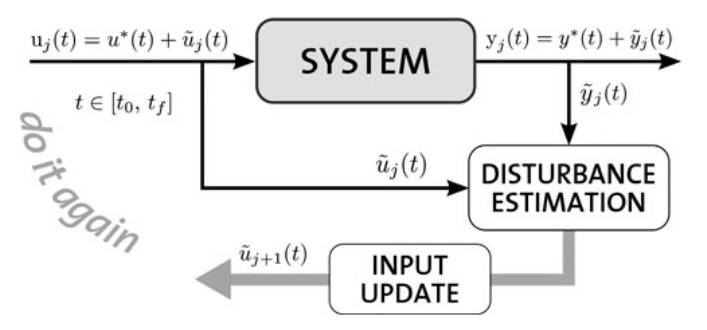
\includegraphics[scale=0.25]{ilc_framework}			
\caption{ILC Framework \cite{ILC_Angela}}
\end{figure}
\end{frame}
%
\begin{frame}{Iterative Learning Control (ILC)}
\begin{itemize}
\item A very simple update rule is to use the error and its derivatives \cite{Arimoto}. For example:
\end{itemize}
\begin{equation*}
\begin{aligned}
\sysInput_{k+1} = \sysInput_{k} + K_{p}(\state_{k} - \traj) + K_{d}(\dot{\state}_{k} - \dot{\traj})
\end{aligned}
\end{equation*}
\end{frame}
%
\begin{frame}{Iterative Learning Control (ILC)}
\begin{itemize}
\item Equivalently we can update the kinematic policy! \cite{Survey}
\item We can update the DMP weights using the same PD update law: 
\end{itemize}
\begin{equation*}
\begin{aligned}
\weights_{k+1} = \weights_{k} + \alpha(\basis^{\mathrm{T}}\basis + \lambda\mathbf{I})^{-1}\basis^{\mathrm{T}}(\state_{k}-\traj)
\end{aligned}
\end{equation*}
\begin{itemize}
\item Or we can update using the forcing term errors:
\begin{equation*}
\begin{aligned}
\weights_{k+1} &= \weights_{k} + \alpha(\basis^{\mathrm{T}}\basis + \lambda\mathbf{I})^{-1}\basis^{\mathrm{T}}(\force_x - \force_r) \\
\force_x &= \ddot{\state} - \alpha_g(\beta_g(g-\state) - \dot{\state}) \\
\force_r &= \ddot{\traj} - \alpha_g(\beta_g(g-\traj) - \dot{\traj})
\end{aligned}
\end{equation*}
\end{itemize}
\end{frame}
%
\begin{frame}{ILC: Pros and Cons}
\begin{itemize}
\item ILC can be more efficient than standard RL approaches: each time step has its own cost $e(t)$, as opposed to using the squared sum of all errors. \pause
\item But ILC is for when you \emph{really} want to track the reference trajectory $\traj(t)$. It assumes that $\traj(t)$ is optimal.
\end{itemize}
\end{frame}
%
\begin{frame}{Optimal Control}
\begin{itemize}
\item For a linear system under a given linear feedback law $\sysInput = -K(\state - \dmp)$ we can write the dynamics as:
\begin{equation*}
\begin{aligned}
 \dot{\fullvec} := \dot{
 \begin{bmatrix}
  \state \\
  \traj \\
  \dmp \\
  g
 \end{bmatrix}} = 
 \begin{bmatrix}
  A_x - B_xK & 0 & BK & 0 \\
  0 & 0 & 0 & \nu(t) \\
  0  & 0  & A_s & A_g  \\
  0 & 0 & 0 & 0
 \end{bmatrix}
 \begin{bmatrix}
   \state \\
   \traj \\
   \dmp \\
   g
  \end{bmatrix} +
  \begin{bmatrix}
    0 \\
    0 \\
    \basis \\
    0
   \end{bmatrix} \weights
\end{aligned}
\end{equation*}
\item We can use LQR to minimize the cost functional:
\begin{equation*}
\begin{aligned}
J(\weights) &= \int_{0}^{T} (\state - \traj)^{\mathrm{T}}Q(\state - \traj) + \weights^{\mathrm{T}}R\weights + (\state_T-\traj_T)^{\mathrm{T}}Q_{T}(\state_T-\traj_T) \\
\weights_{LQR} &= -K_{\weights}(\state - \traj)
\end{aligned}
\end{equation*}
\end{itemize}
\end{frame}
%
\begin{frame}{Optimal Control}
\begin{itemize}
\item This way we end up with dynamic weights for the DMP!
\item We can also introduce the constraint $\dot{\weights} = 0$ to LQR.
\item \todo: Toy example 
\end{itemize}
\end{frame}	
%
\begin{frame}{Connection to ILC}
\begin{itemize}
\item Since we don't know the system matrices $A_x$ and $B_x$, we cannot track the trajectory $\traj(t)$ with this weight-feedback law. \item We can update our weight-feedback law with ILC:
\begin{equation*}
\begin{aligned}
\weights_{new} = \weights_{old} - \alpha(\basis^{\mathrm{T}}\basis + \lambda\mathbf{I})^{-1}\basis^{\mathrm{T}}(\state_{obs} - \traj)
\end{aligned}
\end{equation*}
\item \todo: Show that this is gradient ascent of the cost functional!
\end{itemize}
\end{frame}	
%
\begin{frame}{Conclusion}
\begin{itemize}
\item Thank you for listening!
\end{itemize}
\end{frame}	
%
\section{References}
\begin{frame}[allowframebreaks]{References}
\def\newblock{\hskip .11em plus .33em minus .07em}
\bibliographystyle{alpha}
\bibliography{myReferences} % file name of the bibtex
\end{frame}
%

%
% End of slides
\end{document} 